\section{ NDN Overview\label{ccn-intro}}
Named Data Networking (NDN) is a network architecture which aims to replace IP architecture by replacing IP�s host-to-host data delivery model with pull-based information retrieval model. In IP in order to retrieve data, data consumer have to know endpoint location of the desired data, in NDN all they have to know is data name. Names are hierarchical (non-flat) application-defined string names that are used for forwarding, routing and caching. A canonical NDN name looks in a following way: /ndn/ucla/CSdept/faculty/Lixia/webpage.

NDN communication uses two packet types: Interest and Data. An Interest packet contains data name and is issued by the receiver to express what data is needed. The sender puts a data packet into the network in response to an Interest. An Interest is �satisfied� when a Data packet is received with matching data name.

Every NDN node manages three important data structures:
\begin{enumerate}
\item{Forwarding Interest Base (FIB) maps name prefixes and multiple physical network interfaces (where to forward Interests). Having one-to-many relationship in this table allows multipath forwarding of Interests.}
\item{Content Store (CS) temporarily stores Data packets that pass through this node and allows fast Data retrieval.}
\item{Pending Interest Table (PIT) holds all "not yet satisfied" Interests that have been sent upstream. Every element contains a list of incoming and outgoing physical interfaces to enable multipath Interest forwarding and multipath Data delivery.}
\end{enumerate}

So how it works altogether? Every incoming Interest triggers a lookup in the Content Store and if the Data with matching data name have been found, it is sent back to the same physical interface from which the Interest has arrived. If CS lookup is unsuccessful, Interest must be sent further upstream and put in the PIT. However, all recurring Interests with the same prefix name are stacked together in the same PIT entry and are not sent to the upstream again until this PIT entry expires completely because of timeout. If Data returns from some upstream location it is replicated for each incoming physical interface stored in this PIT entry after that it is removed from PIT. In other words, multipath Data delivery is built-in in NDN. 


%\begin{figure}[htpb]
%  \centering
%  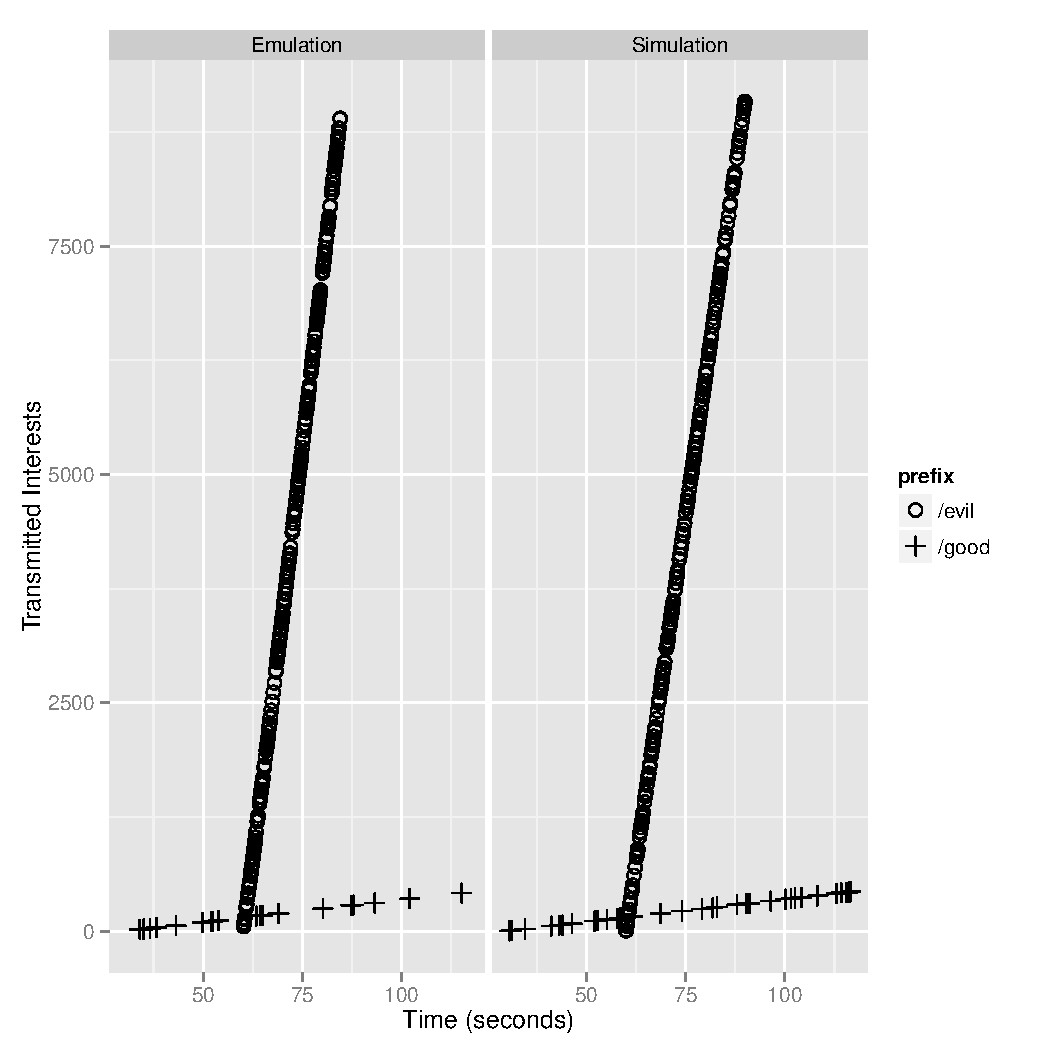
\includegraphics[scale=0.5]{figures/sim-emu-power.pdf}
%  \caption{Strength of Interest flooding attack}
%  \label{fig:simemupower}
%\end{figure}

%\begin{figure}[htpb]
%  \centering
%  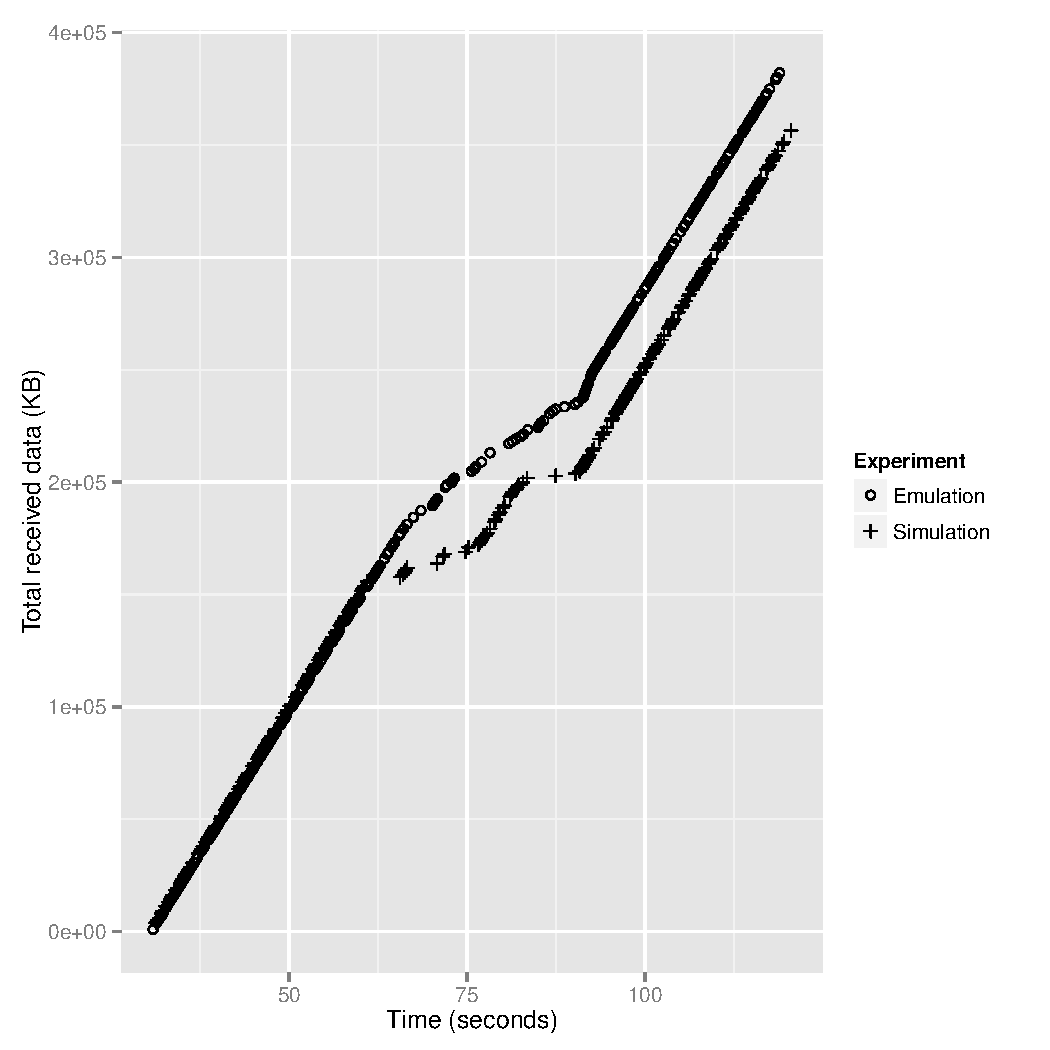
\includegraphics[scale=0.5]{figures/sim-emu-performance.pdf}
%  \caption{Data retrieval by legitimate clients}
%  \label{fig:simemuperf}
%\end{figure}

